\chapter{Teoría de la integración en subvariedades diferenciales}

\section{Repaso: Integración en dimensiones inferiores}

\subsection{Integración en dimensión 1}

En dimensión 1, la teoría de integración la basábamos en la integral de Riemann. Tomábamos una partición de $[a,b]$: $\mathcal{P} = a = t_0 < t_1<...<t_k = b$ y a cada subintervalo de esa partición $I_i =[t_i,t_{i+1}]$ asignábamos dos pares de valores, $M_i$ y $m_i$:

\begin{gather*}
M_i = \sup \{f(x)\tq x\in I_i\}\\
m_i = \inf \{f(x)\tq x\in I_i\}
\end{gather*}

Definíamos las sumas superiores ($\mathbb{U}$) e inferiores ($\mathbb{L}$):

\begin{gather*}
\mathbb{U}(f,\mathcal{P}) = \sum_{i=0}^{k-1} M_i(t_{i+1}-t_i) \\
\mathbb{L}(f,\mathcal{P}) = \sum_{i=0}^{k-1} m_i(t_{i+1}-t_i)
\end{gather*}

Esto nos da una aproximación al área debajo de la función como una suma de rectángulos. Tal y como los hemos definido, está claro que

\[ \mathbb{L}(f,\mathcal{P}) ≤ \int_a^b f ≤ \mathbb{U}(f,\mathcal{P}) \]

También parece obvio que, cuanto más pequeña sea la anchura de los intervalos, más se aproximarán las sumas superiores e inferiores al valor real. Definimos entonces

\begin{gather*}
\alpha = \lim_{\abs{\mathcal{P}}\to 0} \mathbb{U}(f,\mathcal{P}) \\
β = \lim_{\abs{\mathcal{P}}\to 0} \mathbb{L}(f,\mathcal{P})
\end{gather*}

, donde $\abs{\mathcal{P}} = \max t_{i+1} - t-i$, es decir, la anchura máxima de los intervalos que formarn $\mathcal{P}$. A partir de aquí podemos llegar a la definición de función integrable:

\begin{defn}[Función\IS integrable] Se dice que $f$ es integrable en $[a,b]$ si y sólo si

\[ \alpha = \lim_{\abs{\mathcal{P}}\to 0} \mathbb{U}(f,\mathcal{P}) =
\lim_{\abs{\mathcal{P}}\to 0} \mathbb{L}(f,\mathcal{P}) = β \]

La notación es \[ \int_a^b f(x)dx = \alpha = \beta \]
\end{defn}

\begin{theorem}
Si $f$ continua en $[a,b]$ entonces  $f$ es integrable en $[a,b]$.
\end{theorem}

El recíproco es \textbf{falso}. Se ve fácilmente si $f$ es una función escalonada, por ejemplo: podemos calcular el área debajo de ella sin problemas pero no es continua.

\begin{theorem} Sea $f$ integrable en $[a,b]$.

Tomamos $\mathcal{P}_h$ una partición de $[a,b] \tlq \max_{i} \abs{t_{i+1}-t_i} = h$ , es decir, $h$ mide el trozo más grande de la partición.

\[ \lim_{h\rightarrow 0} \sum_{i=1}^{k-1} f(s_i)(t_{i+1}-t_i) = \int_a^bf(x)dx \] para \textbf{cualquier} elección $s_i\in[t_i,t_{i+1}]$

\end{theorem}

\begin{theorem}[Cambio\IS de variable (dimensión 1)]
Sea $g$ un difeomorfismo, y suponemos que es creciente (la cuenta es análoga si fuese decreciente); de tal forma que transforma el intervalo $[a,b]$ en el intervalo $[g(a),g(b)] = [A,B]$. Entonces

\[ \int_A^B f(x)\,dx = \int_{\inv{g}(A)}^{\inv{g}{B}} f(g(t)) g'(t)\,dt \]

Es decir, tenemos cambio de los límites, de las variables y también de la medida.
\end{theorem}

\subsection{Integración en dimensión $1 < N ≤ 3$}

En dimensión mayor que uno teníamos una serie de generalizaciones, y empezábamos con el teorema de Fubini que nos permite el cambio en el orden de integración:

\begin{theorem}[Teorema\IS de Fubini] Sean $A$ y $B$ dos conjuntos compactos. Entonces

\[ \int_A \int_B f(x,y)\,dx\,dy = \int_B \int_A f(x,y)\,dy\,dx \]

En la práctica, tendremos que cambiar los límites de integración para que la integral exprese el mismo área.
\end{theorem}

\begin{wrapfigure}{r}{0.4\textwidth}
\begin{center}
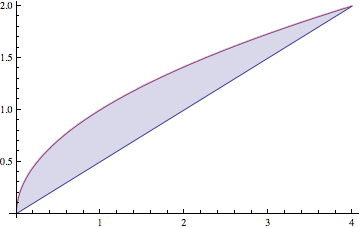
\includegraphics[width=0.4\textwidth]{imgs/AreaInt1.png}
\caption{Integral $I_1$}
\label{imgInt1}
\end{center}
\end{wrapfigure}

Por ejemplo, si tenemos la siguiente integral (ver figura \ref{imgInt1}) \[ I_1 = \int_0^2\int_{y^2}^{2y} f(x,y)\,dx\,dy \] y queremos invertirla cambiamos los límites de integración: \[ I_1 = \int_0^4 \int_{\frac{x}{2}}^{\sqrt{x}} f(x,y)\, dy\,dx \]

Otro ejemplo: estudiemos \[ I_2 = \int_a^bf(x)\,dx = \int_a^b\int_0^{f(x)}dx\,dy \]. Si probamos a cambiar el orden de integración, tenemos que

\[ I_2 = \int_0^M\int_{A(y)}dx\,dy \]

Donde $M$ es el máximo de $f$ y $A(y) = \{ x\in [a,b] \tq f(x) ≥ y \}$. La longitud de ese conjunto $A$ se denomina la medida, y entonces podemos expresar

\[ I_2 = \int_0^\infty \abs{\{x \tq f(x) > y\}}\,dy \] ya que la medida del conjunto será $0$ cuando $y > M$.

Curiosamente, hemos pasado de una integral de Riemann a otra con una expresión distinta, la llamada \textbf{integral de Lebesgue}\index{Integral! de Lebesgue}. Esto pertence al campo de la \textbf{teoría de la medida}, y permite estudiar conjuntos extraños y más monstruos y engendros varios. \label{IntLebesgue}

En general, podemos expresar nuestro cambio de variable de forma más general para cualquier cambio de variable:

\begin{theorem}[Cambio\IS de variable (dimensiones superiores)]
Dados unos conjuntos $D,\,D^\ast$ con $\appl{\Phi}{D}{D^\ast}$ un difeomorfismo, y $\gx \in D;\; \gy \in D^\ast$. Entonces

\[ \int_{D^\ast} f(\gy)\,d\gy = \int_D f(\Phi(\gx)) \abs{\det \dpa{\gy}{\gx}}\,d\gx \]
\end{theorem}

\subsubsection{Integración en curvas}

\begin{defn}[Curva\IS $C^1$]  Se denomina curva en $\real^n$ a una aplicación \begin{align*}
\appl{\gamma}{[a,b]\subset \real&}{\real^n} \\
t&\to \gamma(t) = (x_1(t),\dotsc,x_n(t))
\end{align*}

y con $\gamma\in C^1$.

También exigiremos que la curva sea un \textbf{camino regular}\index{Camino!regular}, es decir que

\[ \gamma'(t) \neq \gor{0} \;\forall t \]

de tal forma que obligamos a que tenga tangente en todo punto.
\end{defn}

Para calcular la longitud aplicamos las ideas básicas del cálculo integral: \textit{troceamos} el intervalo $[a,b]$, y aproximamos cada uno de esos trozos por un segmento. Calculamos la suma de la longitud de esos segmentos, hacemos tender la anchura de los \textit{trozos} y si converge, la longitud se puede medir.

\begin{theorem}[Longitud\IS de una curva] Dada una partición $\mathcal{P} = \{ a= t_0 < t_1 < \dotsb < t_k = b\}$ definimos \[ \abs{\mathcal{P}} = \max_i \abs{t_{i+1} - t_i} \] y la longitud $L$ de la curva.

\[ L(\sigma) = \lim_{\abs{\mathcal{P}}\to 0} \underbrace{\sum_{i=0}^{k-1} \md{\sigma(t_{i+1}) - \sigma(t_i)}}_{=S(\sigma,\mathcal{P})} \]

SI $\sigma\in C^1$, entonces $L(\sigma)$ existe y además

\[ L(\sigma) = \int_a^b \md{\sigma'(t)}\,dt \]

\end{theorem}

Este teorema responde a una idea con respecto al cambio de variable: si tomamos $\Gamma$ como la curva que queremos integrar, entonces se puede expresar

\[ L(\sigma) = \int_\Gamma 1\,d\sigma = \int_a^b \md{\sigma'(t)}\,dt  \]

donde $\md{\sigma'(t)}$ es el cambio en la medida correspondiente.

\begin{proof} Por pura pereza y no escribir más \footnote{A mí también me parece bien} suponemos \[ \sigma(t) = (x(t),y(t)) \]. Tenemos que

\begin{gather*}
 S(\sigma,\mathcal{P}) = \sum_{i=0}^{k-1} \md{\sigma(t_{i+1}) - \sigma(t_i)} = \\
 = \sum_{i=0}^{k-1}\sqrt{\left(x(t_{i+1}-x(t_i)\right)^2 + \left(y(t_{i+1}-y(t_i)\right)^2}
 \end{gather*}

 Por el Teorema del valor medio (\ref{thmTVM1var}) tenemos que

 \begin{gather*}
 \left(x(t_{i+1}-x(t_i)\right)^2  = x'(s_i^1)^2(t_{i+1}-t_i)^2 \\
 \left(y(t_{i+1}-y(t_i)\right)^2  = y'(s_i^2)^2(t_{i+1}-t_i)^2
 \end{gather*}

 Entonces

 \[  S(\sigma,\mathcal{P})  = \sum_{i=0}^{k-1}  (t_{i+1}-t_i) \sqrt{x'(s_i^1)^2 + y'(s_i^2)^2} \]

 No podemos simplificar porque no es seguro que $s_i^1 = s_i^2$. Si fueran el mismo punto, serían sumas de Riemann y habríamos terminado.

 Como tenemos una función continua ($\sigma'$) y estamos trabajando en un intervalo cerrado y acotado ($[a,b]$) podremos reducir la expresión a $\sqrt{x'(t_i)^2 + y'(t_i)^2}$ y que gracias a la continuidad uniforme la diferencia con $\sqrt{x'(s_i^1)^2 + y'(s_i^2)^2}$ se puede hacer todo lo pequeña que queramos, llegando a hacer coincidir en el límite $s_i = t_i$, por lo que podríamos escribir:

\[  S(\sigma,\mathcal{P})  = \sum_{i=0}^{k-1} \sqrt{x'(t_i)^2 + y'(t_i)^2} (t_{i+1}-t_i) \]
  o también:
\[  S(\sigma,\mathcal{P})  = \sum_{i=0}^{k-1} \sqrt{x'(t_{i+1})^2 + y'(t_{i+1})^2} (t_{i+1}-t_i) \]


La forma matemática de escribir este argumento:

Notación: $G(s,t) = \sqrt{(x'(s))^2 + (y'(s))^2}$

Llamamos:
\[(1) = \sum G(s_i^1,s_i^2)(t_{i+1}-t_i)\]
\[(1) = \sum G(t_i^1,t_i^2)(t_{i+1}-t_i)\]

Vamos a estudiar $\abs{(1)-(2)}$

\[0\leq \abs{(1)-(2)} \leq ... \leq \sum_i \abs{G(s_i^1,s_i^2)- G(t_i^1,t_i^2)}(t_{i+1}-t_i)\]

$(s_1^1, s_1^2 \in [t_i,t_{i+1}]$ por tanto:
\[\md{s_i^1,s_i^2) - (t_i,t_i)} = ... \leq \sqrt{2}\md{\mathcal{P}}\]

Aplicamos $G$ continua en $[a,b]\times [a,b]$ (compacto) $\implies G$ uniformemente continua.

\end{proof}

\obs \textbf{Falso} en general si la curva es sólo continua

\paragraph{Ejemplo:}

\[\appl{\sigma}{[0,1]}{\real^2}\]

\todo{A dibujar!}

Descripción gráfica: entre $\frac{1}{2^k}$ y $\frac{1}{2^{k+1}}$ y formo un triángulo isósceles con esos 2 puntos y de altura hasta la bisectriz.

Sea el triangulo K:

\todo{Dibujo}

\[Longitud =L_k = ... ??? ... = \frac{1}{2k+1} \{\sqrt{\frac{1}{4k^2}+1} + \sqrt{\frac{1}{4k^2+4} +1} \} \ge \frac{1}{2k+1}\]
\[\text{Longitud total } = \sum L_k \ge \sum_k \frac{1}{2k+1} = \infty\]

Este mostruito no tiene longitud. ¿Y si en vez de rectas tomamos sinusoides? Esa función si debería ser $C^1$ pero la longitud es $\infty$. Entonces la curva no puede ser $C^1$ (sería un contrajemplo del teorema)

\begin{defn}[Curva\IS rectificable]\label{defCurvaRectf}
Si el límite \[ \lim_{\abs{\mathcal{P}}\rightarrow 0} S(\sigma,\mathcal{P})\] existe entonces $\sigma$ es \textbf{rectificable}.

Además, con comprobar que la curva es $C^1$ es suficiente.

Para que $\sigma$ sea rectificable, basta con que sea continua de Lipschitz, es decir que \[\lim_{x\to x_0} \frac{d(f(x),f(x_0)}{d(x,x_0)}\leq C,\forall x\]

\end{defn}


\subsubsection{Parametrización por longitud de arco}

\[ \appl{\sigma}{[a,b]}{\real^n} \]

con $\sigma$ curva $C^1$ y regular. Entonces

\[ L(s) = \int_a^s \md{\sigma'(t)}\,dt \]

y por el Teorema Fundamental del Cálculo

\[ L'(s) = \md{\sigma'(s)} \]

Al imponer que la curva sea regular, entonces $\sigma'(s)\neq 0$ y por lo tanto existe la inversa $\inv{L}$. Si tenemos entonces un $\tau ∈ [0,L(b)]$, entonces $S=\inv{L}(\tau) ∈ [a,b]$.\wtf

Definimos

\begin{gather*}
\sigma^\ast = \sigma \circ \inv{L} \\
\sigma^\ast = \sigma(\inv{L}(\tau)) \\
(\sigma^\ast)'(\tau) = \sigma'(\inv{L}(tau)) (\inv{L}(\tau))' = \sigma'(\inv{L}(\tau)) \frac{1}{L'(\inv{L}(\tau))} = \sigma'(s) \frac{1}{L'(s)} = \frac{\sigma'(s)}{\md{\sigma'(s)}}
\end{gather*}

Es decir, hemos conseguido una parametrización con velocidad constante $\md{(\sigma^\ast)'} = 1$ y por lo tanto

\[ L(\tau) = \int_0^\tau \md{(\sigma^\ast)'}\,ds = \int_0^s 1\,ds = s \]

\section{Integración en dimensiones superiores}

\subsection{Elemento de área}

Supongamos que estamos en $\real^3$. Podemos hablar de la longitud de una variedad de dimensión 1, del área de una de dimensión 2 o del volumen de una de dimensión 3. Ahora bien, ¿qué ocurre cuando pasamos a dimensiones superiores? La denominación será la siguiente

\begin{itemize}
\item \textbf{1-variedad} Longitud
\item \textbf{k-variedad} $1<k<N$ Área
\item \textbf{N-variedad} Volumen
\end{itemize}

Para calcular esas \textit{cosas} empezaremos partiendo del área de un parelelepípedo.

Definiremos el paralelepípedo como, dados $k$ vectores independientes $\{\gv_i\} \subset \real^N$,

\[ P_k = \sum_{i=1}^k \lambda_i\gv_i\;\lambda_i \in [0,1] \]


Elemento de área: $P_k \equiv \{ \sum_{i=1}^k \lambda_i\gor{v}_i, \lambda_i \in [0,1]\}\subset \real^N$

Definimos una \begin{gather*}
\appl{\Psi}{\real^N}{\real^N}\\
\gx \longrightarrow (\Psi_1(\gx),...,\Psi_n(\gx))
\end{gather*}

\begin{itemize}
\item si $\gx \in P_k \implies \Psi(\gx) = (\Psi_1(\gx),\Psi_2(\gx),...,\Psi_k(\gx),0,...,0)$
\item $\Psi$ mantiene longitudes y ángulos, es decir $\pesc{\Psi(u),\Psi(v)}=\pesc{u,v}, \forall u,v\in\real^N$

Esto implica: $\pesc{\Psi(u),\Psi(v)}=\pesc{u,v} \implies \md{\Psi(\gu)} = \md{\gu}$. Si se conservan los módulos, se conservan también los ángulos.
\end{itemize}

\obs Si $\gx,\gy\in P_k \implies \pesc{\gx,\gy} = \underbrace{\pesc{\Psi(\gx),\Psi(\gy)}}_{\text{Prod } \real^N} = \underbrace{{\tilde{\Psi}(\gx),\tilde{\Psi}(\gy)}}_{\text{Prod } \real^K}$


\textbf{Idea:} Área $(P_k)$ = Área $(\tilde{\Psi}(P_k)) \equiv \displaystyle \int_{\tilde{\Psi}(P_k)}d\gor{s}$, una integral en $\real^K, K<N$



El paso que vamos a dar ahora es: Construir una aplicación $L$ tal que $L(\gor{e}_i) = \tilde{\Psi}(\gor{v}_i)$

Y aplicamos el cambio de variables:
\[\int_{\tlps(P_k)} d\gor{s} = \int_{[0,1]^K} \abs{\det\left( \dpa{s}{t} \right)} d\gor{t}\]

Tenemos:
\begin{itemize}
\item $L$ lineal, $\appl{L}{\real^K}{\real^K}$
\item $L(\gor{e}_j) = \tlps(\gv_j)$.
\end{itemize}
Con la segunda propiedad podemos construir la aplicación $L$.

\begin{gather*}
L = \begin{pmatrix} \tlps(\gv_1) & \tlps(\gv_2) & ... & \tlps(\gv_k)\\
\downarrow & \downarrow & \ddots & \downarrow
\end{pmatrix} = \frac{d\gor{s}}{d\gor{t}}\end{gather*}

\textbf{Conclusión:} \[Area(P_k) = \abs{\det L} = \left|\det \begin{pmatrix}
\tlps(\gv_1) & \tlps(\gv_2) & ... & \tlps(\gv_k)\\
\downarrow & \downarrow & \ddots & \downarrow
\end{pmatrix}\right|\]

Pero... tenemos 2 problemas:
\begin{itemize}
\item Necesitamos una manera cómoda con la que construir $\tlps$.
\item ¿Utilizando otra parametrización llegamos al mismo resultado?
\end{itemize}

Vamos a reventar 2 pajaros de un tiro.

\[ Area(P_k) = \left( \det \begin{pmatrix}
\tlps(\gv_1) & \tlps(\gv_2) & ... & \tlps(\gv_k)\\
\downarrow & \downarrow & \ddots & \downarrow
\end{pmatrix}
\begin{pmatrix}
\tlps(\gv_1) & \tlps(\gv_2) & ... & \tlps(\gv_k)\\
\downarrow & \downarrow & \ddots & \downarrow
\end{pmatrix} ^T \right)^{\frac{1}{2}}\]
¿Qué ganamos?
\[\begin{pmatrix}
\pesc{\tlps(\gv_1),\tlps(\gv_1)} & \pesc{\tlps(\gv_1),\tlps(\gv_2)} & ... & \pesc{\tlps(\gv_1),\tlps(\gv_k)}\\
\pesc{\tlps(\gv_2),\tlps(\gv_1)} & \pesc{\tlps(\gv_2),\tlps(\gv_2)} & ... & \pesc{\tlps(\gv_2),\tlps(\gv_k)}\\
\vdots & \vdots & \ddots & \vdots\\
\pesc{\tlps(\gv_k),\tlps(\gv_1)} & \pesc{\tlps(\gv_k),\tlps(\gv_2)} & ... & \pesc{\tlps(\gv_k),\tlps(\gv_k)}
\end{pmatrix} = (\ast) = \left(\det(\pesc{v_i,v_j})\right)^{\frac{1}{2}}\]
($\ast$) Hemos construido las cosas de tal manera que se mantiene el producto escalar.

\paragraph{Ejemplo: } $P_2 \subset \real^3$ generado por $\gu,\gv\in\real^2$

$Area(P_2) = \left(\det \begin{pmatrix}
\pesc{\gu,\gu} & \pesc{\gu,\gv}\\
\pesc{\gv,\gu} & \pesc{\gv,\gv}
\end{pmatrix} \right)^{\frac{1}{2}} = \left(\pesc{\gu,\gu}\pesc{\gv,\gv} - \pesc{\gu,\gv}^2\right)^{\frac{1}{2}} =\left(\md{\gu}\md{\gv} - \md{\gu}\md{\gv}(cos(\theta)^2)\right)^2 = \md{u}\md{v} \sqrt{1-cos^2(\theta)}  =  \md{u}\md{v} sen(\theta) = ||u\times v||$

Bueno, esto cumple lo que la sabíamos de selectividad. El área de un paralelogramo 2 dimensional en $\real^3$ es la raiz cuadrada del módulo del producto vectorial.

\textbf{Aplicación:} Vamos a aplicar esto para hallar el área de una $k-variedad$ en $\real^N$.

\todo{Dibujo}
\begin{itemize}
\item $\Phi(\gs_0) = \gx_0 \in M$
\item $\Phi(\gs_0 + h_j\gor{e}_j) = \Phi(\gs_0) + \dpa{\Phi}{s_j}(\gs_0)\cdot h_j + err(h)$
Aplicando taylor, en el que cada alargamiento $h$ depende de la dirección.
\end{itemize}

\textbf{Idea:} $Area(\Phi(Q_k)) = Area(P_k) + err(h)$ donde $Area(P_k) = \left(\det (\pesc{v_i,v_j})\right)^{\frac{1}{2}}, \{v_j\}$ genera $P_k$.

\todo{Me he perdido porque $v_i = \dpa{\Phi}{s_j}(\gs_0)\cdot h_j$}

\[\left(\det\left(\pesc{\dpa{\Phi}{s_i},\dpa{\Phi}{s_j}}h_ih_j\right)\right)^{\frac{1}{2}}\]

Tomamos $h_i = h, \forall i$

\[\underbrace{\underbrace{h^k}_{Area(Q_k)} \left(\det\left(\pesc{\dpa{\Phi}{s_i},\dpa{\Phi}{s_j}}\right)\right)^{\frac{1}{2}}}_{Area(P_k)}\]

Conclusión: \[Area(M) = \sum_n Area(Q_k^n) \left(\det\left(\pesc{\dpa{\Phi}{s_i}(\gs_0^n),\dpa{\Phi}{s_j}(\gs_0^n)}\right)\right)^{\frac{1}{2}} + err(h)\]

Si llamamos $F(s_0^n) = \left(\det\left(\pesc{\dpa{\Phi}{s_i}(\gs_0^n),\dpa{\Phi}{s_j}(\gs_0^n)}\right)\right)^{\frac{1}{2}}$

Tenemos: \[\sum_n Area(Q_k) F(s_0^n) \convs[Riemann] \int_D F(\gs)d\gs\]

\textbf{Por tanto:} $Area(M) = \int_D \left(\det\left(\pesc{\dpa{\Phi}{s_i},\dpa{\Phi}{s_j}}\right)\right)^{\frac{1}{2}}$

Lo que en Cálculo 2 llamábamos $\md{T_u\times T_v}$.


Dada una $\appl{f}{\real^N}{\real}$ podemos definir: \[\int_{\Phi(D)}f dA = \int_{D}f(\Phi(s)) \left(\det(\pesc{\Phi_{s_i},\Phi_{s_j}})\right)^{\frac{1}{2}} ds\]

\paragraph{Ejemplos}

\subparagraph{Ejemplo 1)}

\[\appl{\sigma}{[a,b]}{\real^N}\]

Sea $\Gamma = \{\sigma(t)\in\real^N\tq t\in[a,b]\}$

El elemento de área sería:

\[\int_{\Gamma} fdA = \int_a^bf(\sigma(t)) (\pesc{\sigma',\sigma'})^{\frac{1}{2}}\]


\subparagraph{Ejemplo 2)}

\[
\Phi : D\subset\real^2\rightarrow \real^3\]
\[(s_1,s_2)\rightarrow (x(s_1,s_2),y(s_1,s_2),z(s_1,s_2))\]

Tenemos en este caso:
\[\int_{\Phi(D)}fdA = \int_D f(\Phi(s_1,s_2)) (\det(\pesc{\Phi_{s_i},\Phi_{s_j}}))^{\frac{1}{2}})ds\]
\[(\det(\pesc{\Phi_{s_i},\Phi_{s_j}}))^{\frac{1}{2}}) = (*) = \md{\Phi_1 \times \Phi_2}\]
$(*)$ visto anteriormente.

Integrales de \textbf{campos} sobre \textbf{curvas} y \textbf{superficies} en $\real^3$.

\begin{itemize}
\item[1] $\Gamma$ curva, $\overrightarrow{F}$ campo. Nos interesa la componente que sigue la tangente de la recta (ya que en la dirección perpendicular no se realiza trabajo). Para ello multiplicamos escalarmente por el vector director normalizado.
\[\int_{\Gamma} \overrightarrow{F}d\sigma \equiv \text{ Trabajo } \equiv \int_{\Gamma} F_T = \int_{\Gamma} \pesc{\overrightarrow{F},\frac{\sigma'}{\md{\sigma'}}}\]
\[ = \int_a^b \pesc{\overrightarrow{F}(\sigma(t)),\frac{\sigma'(t)}{\md{\sigma'(t)}}} \md{\sigma'(t)}dt = \int_a^b \pesc{\overrightarrow{F}(\sigma(t)),\sigma'(t)} dt\]

\item[2] Flujo a través de una superficie.

En este caso, la componente que nos interesa es la perpendicular a la superficie.

$\overrightarrow{n} = T_u\times T_v$

\[\int_{\Phi(D)} \overrightarrow{F} = ... = \int_{D} \pesc{\overrightarrow{F}(\Phi(u,v)),T_u\times T_v}dudv\]
\end{itemize}

Volvemos a plantearnos el problema: ¿Distintas parametrizaciones nos da el mismo trabajo/flujo? Depende de la \textit{orientación} de la parametrización. No es lo mismo el trabajo para ir desde abajo de la curva hasta arriba que para bajarla. ¿Este problema traducido a $\real^K$, flipas o k ase?


Recordamos algunos teoremas y definiciones vistos en Calculo 2:

\subsection{Campos vectoriales}
Los campos vectoriales son funciones $\appl{F}{\real^N}{\real^N}$, en el que a cada punto se le asigna un vector.
\index{Campo!vectorial}

\begin{defn}[Campo\IS conservativo]
Diremos que $F$ es un campo gradiente o conservativo si $\exists \appl{V}{\real^N}{\real}$ tal que $F=\nabla V$.
\end{defn}

\begin{defn}[Divergencia]
En un campo vectorial, la divergencia mide el cambio de volumen y existencia de fuentes o sumideros. Si la divergencia es 0, tenemos un "fluido" incompresible.

\[ \textrm{div}\;F = \frac{∂F_1}{∂x_1} + \cdots + \frac{∂F_n}{∂x_n} \]
\end{defn}

\begin{defn}[Rotacional]
El rotacional mide el giro interno de las partículas en un campo, que se puede expresar como \footnote{En realidad, $\nabla$ no es un vector y esto es sólo una regla mnemotécnica}

\[ \textrm{rot}\;F = \nabla \x \vf \]

Si el rotacional es distinto de cero, significa que ha habido choques internos de las partículas y por lo tanto ha habido pérdida de energía.
\end{defn}

\begin{theorem}
Supongamos que $F\in C^1$ es un campo gradiente. Entonces, $\rot F = \vec{0}$. El recíproco también es cierto.
\end{theorem}


\begin{theorem}[Teorema\IS de Green]
Sea $\Gamma$ una curva simple en $\real^2$. Llamamos $D$ al interior de $\Gamma$. Sea $(P,Q)$ el campo con $P,Q\in C^1(D)$. Entonces

\[ \int_{\Gamma^+} (P,Q)\dif \sigma = \iint_D \frac{\partial Q}{\partial x}-\frac{\partial P}{\partial y}\id{x,y} \]
\end{theorem}

\begin{theorem}[Teorema\IS de Stokes]
Dada $\Gamma$ una curva cerrada simple en $\real^3$ que es el borde de una superficie $S$, tenemos que

\[ \int_{\Gamma^+}\vec{F}\dif \sigma =\iint_{S^+}\rot \vec{F}\dif S \]

Esto indica que el flujo por una superficie depende sólo de la forma de su boca.
\end{theorem}

\begin{theorem}[Teorema\IS de Gauss]
Sea $S$ una superficie cerrada que encierra una región $\Omega$, y $\vec{F}\in C^1(\Omega)$.

\[ \iint_{S^+} \vf \dif S = \iiint_\Omega \dv \vec{F}\, \id{x,y,z} \]
\end{theorem}


Todos estos teoremas son parecidos en cuanto a que a la izquierda se tiene el campo evaluado en la frontera y a la derecha tenemos una integral en el interior de una expresión más o menos compleja en la que aparecen las derivadas. Cabe esperar que sean casos particulares de un teorema superior, cosa que es cierta. Este teorema se le llama de \textbf{Stokes} en general.

De aquí al final de curso nos dedicaremos a llegar a ese teorema y ver que estos 3 teoremas son casos particulares.

Para ello nos adentraremos en el espinoso jardín de la orientación.

\subsection{Orientación}
El tema de la orientación tiene que ver con tener cuidado con el orden. Vamos a ver los ejemplos de pocas dimensiones:

\paragraph{Ejemplos:}

\subparagraph{Ejemplo 1) Bases en $\real^2$}

\[\mathcal{B}_1 = \{(0,1),(1,0)\}\]
\[\mathcal{B}_2 = \{(1,0),(0,1)\}\]

Sea $\gv = (v_1,v_2)_{\mathcal{B}_1} = (v_2,v_1)_{\mathcal{B}_2} \neq \gv$

Lo que haremos en este caso será un cambio de base, $\mathcal{B}_1,\mathcal{B}_2$ bases en $\real^N$. Sea $\mathcal{C}_{\mathcal{B}_1\to\mathcal{B}_2}$ matriz del cambio de base de $\mathcal{B}_1$ a $\mathcal{B}_2$.

\begin{defn}[Orientación]
Diremos que $\mathcal{B}_1,\mathcal{B}_2$ tiene la misma orientación $\dimplies \det \mathcal{C}_{\mathcal{B}_1\to\mathcal{B}_2} > 0$
\end{defn}

¿Que pasaría si el determinante de esa matriz de cambio de base sea 0? No puede ser (por definición de cambio de base, que tiene que ser reversible).

\subparagraph{Ejemplo 2)} $\real^3$.
Sean
\[\mathcal{B}_1 = (\gu,\gv,\gw),\mathcal{B}_2 = (\gv,\gu,\gw),\mathcal{B}_3 = (\gw,\gu,\gv)\]

Si tomamos $\gu = \begin{pmatrix} 1\\0\\0\end{pmatrix}_{\mathcal{B}_1} = \begin{pmatrix}0\\1\\0\end{pmatrix}_{\mathcal{B}_2} = \begin{pmatrix}0\\1\\0\end{pmatrix}_{\mathcal{B}_3} $

Siguiendo este razonamiento llegamos a la matriz de cambio de base:

\[\mathcal{C}_{\mathcal{B}_1\to\mathcal{B}_2} = \begin{pmatrix} 0 & 1 & 0 \\ 1 & 0 & 0 \\ 0 & 0 & 1 \end{pmatrix}\]
Cuyo determinante es negativo.

Lo mismo con

\[\mathcal{C}_{\mathcal{B}_1\to\mathcal{B}_1} = \begin{pmatrix} 0 & 0 & 1 \\ 1 & 0 & 0 \\ 0 & 1 & 0 \end{pmatrix}\]
Cuyo determinante es positivo.

¿Porqué al cambiar el orden se cambia la orientación?

\obs Aceptamos como orientación positiva la de la base canónica ordenada como Dios manda: $\{(1,0,0,...,0), (0,1,0,0,...,0), (0,0,1,0,0,...,0),...,(0,0,...,0,1)\}$

Vamos con algún ejemplo más:

\subparagraph{Ejemplo 3)} (Importante)

En $\real^3$, sean $\gu,\gv$ independientes.

Construimos $\mathcal{B} = \{\gu,\gv,\gu\times\gv\}$. Queremos saber si esta base es de orientación positiva u orientación negativa.

\[\gu\times\gv = \left|
\begin{array}{ccc}
 \overrightarrow{i} & \overrightarrow{j} & \overrightarrow{k}\\
u_1 & u_2 & u_3 \\
v_1 & v_2 & v_3
 \end{array}\right| = ... = \left(\left|\begin{array}{cc}u_2&v_2\\u_3&v_3\end{array}\right|,\left|\begin{array}{cc}u_1&v_1\\u_3&v_3\end{array}\right|,-\left|\begin{array}{cc}u_1&v_1\\u_2&v_2\end{array}\right|\right)\]

 \[\mathcal{B}_{\mathcal{B}\to\mathcal{C}} = \begin{pmatrix}
u_1&v_1& \left|\begin{array}{cc} u_2&v_2\\u_3&v_3 \end{array}\right|\\

u_2&v_2& -\left|\begin{array}{cc} u_1&v_1\\u_3&v_3 \end{array}\right|\\

u_3&v_3& \left|\begin{array}{cc} u_1&v_1\\u_2&v_2\end{array}\right|
 \end{pmatrix}\]

 Cuyo determinante es \[\left|\begin{array}{cc}u_2&v_2\\u_3&v_3\end{array}\right|^2+\left|\begin{array}{cc}u_1&v_1\\u_3&v_3\end{array}\right|^2+\left|\begin{array}{cc}u_1&v_1\\u_2&v_2\end{array}\right|^2>0\]


\subparagraph{Ejemplo 4)} $\real^2$

Sean \[\mathcal{C} = \{(1,0),(0,1)\}\]
\[\mathcal{B} = \{(u_1,u_2),(v_1,v_2)\}\]

La matriz fácil de calcular es \[C_{\mathcal{B}\to \mathcal{C}} = \begin{pmatrix} u_1&v_1\\u_2&v_2\end{pmatrix}\]
\[0<\det \begin{pmatrix} u_1&v_1\\u_2&v_2\end{pmatrix}  = \pesc{(u_1,u_2),(v_1,v_2)} = \pesc{(\lambda,0),(\beta,-\alpha)} = \lambda\beta\]

Aplicando un giro (de aquí salen $\lambda$...) podemos ver que el si el ángulo entre $\gu,\gv \in (0,\pi) \leadsto +$ pero si el ángulo entre $\gu,\gv \in (\pi,2\pi) \leadsto -$. ¿Y en $\pi$? Entonces los vectores no serían independientes.

\textbf{Idea:} Vamos a dedicarnos a jugar con los vectores de la base aplicandoles una deformación continua para ver que pasa con la discontinuidad de la orientación en $\pi$ a ver que encontramos.

Sea la deformación $(\alpha(t),\beta(t)), t\in(0,1)$ continua, donde $(\alpha(0),\beta(0)) = (e_1,e_2)$ y $(\alpha(1),\beta(1)) = (e_1,e_2)$

\begin{itemize}
\item
Si la orientación de la base que tengo al final es positiva, entonces podemos encontrar una transformación continua que mantenga positivo el determinante, $\forall t$.
\item
Si la orientación es negativa, entonces \textbf{siempre} det=0 para algún $t$.
\end{itemize}

\paragraph{Vamos a extender la idea anterior} en $\real^3$.

Idea geométrica: Yo tengo 2 bases y quiero pasar de una a otra, si puedo encontrar un camino en el que los 3 vectores nunca pertenezcan al mismo plano entonces la orientación es la misma. \textbf{El orden es fundamental}.

Sea
\[\mathcal{B} = \{e_1,e_2,e_3\} \hspace*{150pt} \mathcal{C} = \{\gu,\gv,\gw\}\]


\hspace*{50pt}
\begin{tikzpicture}[baseline=(X.base)]
\def\R{2.5} % sphere radius
\def\angEl{15} % elevation angle
\def\angAz{-105} % azimuth angle
\def\angPhi{-40} % longitude of point P
\def\angBeta{19} % latitude of point P


%Ecuador
\pgfmathsetmacro\H{\R*cos(\angEl)} % distance to north pole

\tikzset{xyplane/.estyle={cm={cos(\angAz),sin(\angAz)*sin(\angEl),-sin(\angAz),
                              cos(\angAz)*sin(\angEl),(0,0)}}}
\draw[xyplane,<->] (3,0) node[below] {$e_1$} -- (0,0) -- (0,3)
    node[right] {$e_2$};
\draw[->] (0,0) -- (0,3) node[above] {$e_3$};

\end{tikzpicture}
\hspace*{100pt}
\begin{tikzpicture}[baseline=(X.base)]

\def\R{2.5} % sphere radius
\def\angEl{15} % elevation angle
\def\angAz{-105} % azimuth angle

\tikzset{xyplane/.estyle={cm={cos(\angAz),sin(\angAz)*sin(\angEl),-sin(\angAz),
                              cos(\angAz)*sin(\angEl),(0,0)}}}
 \draw[xyplane,<->] (3,0) node[below] {$\gu$} -- (0,0) -- (0,3)
    node[right] {$\gv$};
\draw[->] (0,0) -- (0,-3) node[right] {$\gw$};
\end{tikzpicture}

No hay ninguna manera de llevar $e_3$ a $\gw$ sin formar un único plano con los tres vectores.

Aunque podríamos llevar $e_3 \to \gu$ y $e_1 \to \gw$... ¿Entonces?

Mal! Porque no estamos manteniendo el orden, tendríamos la base $\mathcal{C}* = \{\gw,\gv,\gu\}\neq\mathcal{C}$.


\paragraph{Caracterización práctica}
\begin{lemma}
\label{thmProdVect} Si $\gu,\gv$ son vectores independientes, entonces $\{ \gu,\gv,\gu\times\gv \}$ es una base.
\end{lemma}

\begin{lemma} La base $\{\gu,\gv,\gw\}$ tiene orientación positiva si y sólo si $\gw$ y $\gu\times\gv$ están en el mismo lado del espacio respecto del plano generado por $\gu,\gv$ (o, lo que es lo mismo, $\pesc{\gw,\gu\x\gv} > 0$).
\end{lemma}

Ahora que ya tenemos vista la orientación de bases en $\real^N$ vamos a ver la orientación en $T_a M$ (espacio tangente de una variedad en un punto)

\todo{Tipico dibujo de un conjunto en el plano $\real^K$ que la parametrización $\Phi$ lo lleva al espacio.}

Sea $\{e_1,e_2,\dotsc,e_k\}$ la base canónica en $\real^k$, y $\Phi(u_0)=\ga$

Como la variedad viene dada por una parametrización, tomamos $\img D\Phi$, es decir: \[T_{\ga}M = \img D\Phi(u_0)  = \{D\Phi(u_0)\gv,\gv\in\real^K\}\]
Tomando la base euclídea:
\[D\Phi(u_0) \{\sum^k v_i\gor{e}_i\}\equiv \sum^k v_i\underbrace{[D\Phi(u_0)\gor{e}_i]}{\in\real^N} \]

\subparagraph{1)}Es decir, la $\img D\Phi$ está generada por los k vectores \begin{equation}\label{baseTaM}
\{ D\Phi(u_0)\gor{e}_1,\dotsc ,D\Phi(u_0)\gor{e}_k \}
\end{equation}

\subparagraph{2)}
La condición de rango máximo nos asegura que los $k$ vectores son linealmente independientes.

\paragraph{Conclusión:} El conjunto (\ref{baseTaM}) es una base de $T_{\ga}M$

\textit{Problema} Si tenemos 2 parametrizaciones distintas $\Phi,\Psi$ entonces tendremos 2 bases diferentes. Cabe plantearse bajo qué condiciones se mantiene la orientación. (aunque todavía no tengamos muy claro que es la orientación de una variedad)

\paragraph{Ejemplos:}
\subparagraph{1)} Las orientaciones de una curva en $\real^N$ es fácil, basta comprobar los sentidos de los vectores tangentes.

Vamos a hacer las cuentas:

Sean $\sigma,\beta$ parametrizacones del mismo trozo de la curva, que parten de orígenes distintos.

\[\appl{\sigma}{U}{\Gamma},s\to \sigma(s)\]
\[\appl{\beta}{V}{\Gamma},t\to \beta(t)\]

Tenemos un teorema que nos garantiza que existe un \textbf{difeomorfismo} (\ref{TeoremaDifeomorfismo})g, tal que \[\sigma(s) = \beta(g(s)) \y \sigma'(s) = \beta'(g(s))\cdot g'(s)\]

En este caso, para que las dos parametrizaciones den la misma orientación, $g'>0$.

\subparagraph{2)} Las orientaciones de una superficie también, basta comprobar los sentidos de los vectores normales.

\[\appl{\Phi}{U}{\real^3}, (u,v) \to \Phi(u,v)\]
\[\appl{\Psi}{V}{\real^3}, (r,s) \to \Psi(r,s)\]

Tenemos un teorema que nos garantiza... tal que \[g(u,v) = (g_1(u,v),g_2(u,v))\]

En este caso, calculamos \[\left.\begin{array}{c}
\Phi_u\times\Phi_v \\
\Psi_r\times\Psi_s
\end{array}\right\}\]

Tenemos que $\Phi(u,v) = \Psi(g_1(u,v),g_2(u,v))$

\begin{gather*}
\Phi_1(u,v) = \Psi_1(g_1(u,v),g_2(u,v))\\
(\Phi_1)_{u} = (\Psi_1)_r r_u + (\Psi_1)_s s_u = ((\Psi)_r\,(\Psi_1)_s)\begin{pmatrix}
(g_1)_u\\(g_2)_v
\end{pmatrix}
\end{gather*}
Se calculan las 6 derivadas $(\Phi_1,\Phi_2,\Phi_3)$ respecto de $u$ y de $v$ \emph{Teniendo cuidado de en donde evaluamos que derivadas} y acabamos llegando a

\[\begin{pmatrix}
(\Phi_1)_u\\(\Phi_2)_u\\(\Phi_3)_u
\end{pmatrix} = \begin{pmatrix}
(\Psi_1)_r & (\Psi_1)_s\\
(\Psi_2)_r & (\Psi_2)_s\\
(\Psi_3)_r & (\Psi_3)_s
\end{pmatrix}\begin{pmatrix}
(g_1)_u\\
(g_2)_u
\end{pmatrix}
\]
Análogamente:
\[\begin{pmatrix}
(\Phi_1)_v\\(\Phi_2)_v\\(\Phi_3)_v
\end{pmatrix} = \begin{pmatrix}
(\Psi_1)_r & (\Psi_1)_s\\
(\Psi_2)_r & (\Psi_2)_s\\
(\Psi_3)_r & (\Psi_3)_s
\end{pmatrix}\begin{pmatrix}
(g_1)_v\\
(g_2)_v
\end{pmatrix}
\]

Ahora procedemos a calcular
\[\Phi_u\x\Phi_v = \dotsc = \left(
\left|\begin{array}{cc}
(\Phi_2)_u & (\Phi_2)_v\\
(\Phi_3)_u & (\Phi_3)_v
\end{array}
\right|,-
\left|\begin{array}{cc}
(\Phi_1)_u & (\Phi_1)_v\\
(\Phi_3)_u & (\Phi_3)_v
\end{array}
\right|,
\left|\begin{array}{cc}
(\Phi_1)_u & (\Phi_1)_v\\
(\Phi_2)_u & (\Phi_2)_v
\end{array}
\right|
\right)\]

Tomando el primer elemento calculamos:

\[
\det\left(
\begin{array}{cc}
(\Psi_2)_r & (\Psi_2)_s\\
(\Psi_3)_r & (\Psi_3)_s
\end{array}
\right)\begin{pmatrix}
(g_1)_u &(g_1)_v \\
(g_2)_u & (g_2)_v
\end{pmatrix} =
\left| \begin{array}{cc}
(\Psi_2)_r & (\Psi_2)_s\\
(\Psi_3)_r & (\Psi_3)_s
\end{array}\right| \det Dg
\]

Repitiendo la cuenta con el resto de los elementos, llegamos a

\[\Phi_u\x\Phi_v = \Psi_r\x\Psi_s\cdot (\det Dg)\]

\paragraph{Conclusión} Para mantener la orientación necesitamos $\det Dg > 0$

\begin{defn}[Orientación \IS en $\real^N$]
Sean $\Phi,\Psi$ parametrizaciones de una subvariedad k-dimensional en $\real^N$, con $g \equiv$ cambio de variables tal que $\Phi=\Psi \circ g$.
Entonces $\Phi,\Psi$ inducen la misma orientación $\dimplies \det Dg>0$
\end{defn}

\obs Este teorema solo afecta a la zona de la subvariedad $M$ parametrizada por $\Phi$ y $\Psi$ al mismo tiempo.

\paragraph{Ejemplo de superficies no orientables}

\subparagraph{Banda de Moebius}
\begin{center}
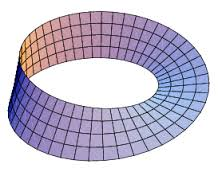
\includegraphics[width=0.5\textwidth]{imgs/Moebius.jpg}
\end{center}
\index{Banda de Moebius}


La parametrización es
\[
\Phi(t,\theta) = \left((R+t\cdot sen\frac{\theta}{2})cos\theta, (R+t\cdot sen\frac{\theta}{2})sen\theta, t cos\frac{\theta}{2} \right) \, t\in(-1,1),\theta\in(0,2\pi)
\]

¿Estamos seguros de que es una parametrización?
\begin{itemize}
\item Regular ($C^1$)
\item $D\Phi$ rango máximo (Fácil)
\item Homeomorfismo
\end{itemize}

Vamos a comprobar el homeomorfismo,

Tenemos 2 posibles caminos:

\subparagraph{1)} Despejamos  en función de $x,y,z$

$\frac{y}{x} = tg \theta$.

Definimos \footnote{Utilizando: (\ref{ImgCirc2})}: \[
\begin{array}{ccc}
\theta &= arctg\frac{y}{x} & (1)\\
\theta &= arctg\frac{y}{x} + \pi & (2)\\
\theta &= arctg\frac{y}{x} + 2\pi & (3)
\end{array}
\]
Y comprobar que es continua


\subparagraph{2)} Escribimos este conjunto como un conjunto de nivel y ver que es una variedad, por lo tanto no hace falta comprobar el homeomorfismo sobre la imagen.

\begin{gather*}
\sqrt{x^2+y^2} = (R + t\cdot cos\frac{\theta}{2})\\
\sqrt{x^2+y^2} - R = \frac{z}{tg\frac{"arctg\frac{y}{x}"}{?}}
\end{gather*}


\subparagraph{Orientación}

Una clave importante es que cuando $\theta\rightarrow 0^+ \implies \Phi(t,\theta)$ pero si $\theta\rightarrow 2\pi^{-} \implies \Phi(-t,\theta)$

$\overrightarrow{n} = T_t\x T_{\theta} = ... = \overrightarrow{n}(t,\theta)$

\begin{gather*}
\overrightarrow{n}(t,\theta) \convs[][\theta\rightarrow 0^+] (-R,\frac{t}{2})\\
\overrightarrow{n}(t,\theta) \convs[][\theta\rightarrow 2\pi^-] (R,-\frac{t}{2})
\end{gather*}

Curioso: esta parametrización que no cubre el segmento con el que se empieza. Esta parametrización tiene una propiedad curiosa, al empezar, el vector normal apunta hacia dentro y al final, apunta hacia fuera. Es imposible cubrirla del todo con una parametrización.

\paragraph{El otro ejemplo} típico de superficie no orientable es la botella de Klein

\begin{center}
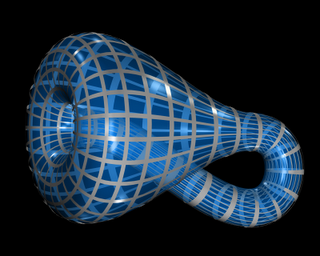
\includegraphics[width=0.5\textwidth]{imgs/botella-de-klein.png}
\end{center}


\paragraph{Variedades con borde}

Conjuntos con frontera en $\real^2$.

Utilizamos la tercera caracterización de subvariedad, que dice que existe un \textbf{difeomorfismo} que vamos a llamar $\Phi$, (que por ser difeomorfismo, existe $\Psi = \Phi^{-1})$.

Podemos suponer que estamos trabajano con un cuadrado en el plano y su imagen para facilitar las cuentas.

Partimos de \begin{itemize}
\item $\Psi(s_0,0) = (x_0,y_0)\in dM$ (la frontera de $M$)
\item $\Psi(s_0,0) \in dM$
\item $\Psi(s,t) \in M, t>0 (s,t)\in U$
\end{itemize}

En U es fácil orientar un cuadrado. ¿Cómo nos "llevamos" la orientación? Con la diferencial, que si queremos que sea la misma orientación $\implies \det D\Phi > 0$.

Sea $\mathcal{C} = \{e_1=(1,0),e_2=(0,1)\}$ base canónica en $\real^2$ (variables (s,t)).

Sea $\mathcal{B} = \{D\Psi(s_0,0)e_1,D\Psi(s_0,0)e_2\}$ base en $\real^2$ (variables $(x,y)$)

Tenemos también $\sigma(s) = \Psi(s,0)$ parametrización de un trozo de $dM$ que contiene a $x_0$.

\[D\Psi = \begin{pmatrix}
\displaystyle\dpa{\Psi_1}{s} &\displaystyle\dpa{\Psi_1}{t}\\
\displaystyle\dpa{\Psi_2}{s} &\displaystyle\dpa{\Psi_2}{t}
\end{pmatrix}\]
En la primera columna lo que tenemos es el vector tangente a la curva. Cuando $t=0$ tenemos la parametrización de la frontera.

\[
D\Psi|_(s_0,0) = \begin{pmatrix}
\sigma'(s_0) & \overrightarrow{v}\\
\downarrow & \downarrow
\end{pmatrix}
\]

Haciendo un desarrollo de Taylor tenemos:

\[
\Psi(s_0,t) = \begin{pmatrix}
\Psi_1(s_0,0)\\
\Psi_2(s_0,0)
\end{pmatrix} + t \underbrace{\begin{pmatrix}
\dpa{\Psi_1}{t} (s_0,0)\\
\dpa{\Psi_2}{t} (s_0,0)
\end{pmatrix}}_{\gor{v}} + err
\]

\[\underbrace{\begin{pmatrix}\Psi_1(s_0,t)\\
\Psi_2(s_0,t)
\end{pmatrix} }_{\in M\, t>0}= \gor{x}_0 + t\gv + err
\]
Conclusión: $\gv$ "apunta hacia el interior de $M$".

\subparagraph{Orientación}
\[\mathcal{C} = \{e_1,e_2\}\]
\[\mathcal{B} = \{D\Psi(s_0,0)e_1,D\Psi(s_0,0)e_2\} = \{\sigma'(s_0),\gv\}\]

\[\mathcal{B} \text{ orientación positiva } \dimplies \det D\Psi(s_0,0) > 0 \dimplies \text{ Ángulo entre } \sigma'(s_0) \text{ y } \gv \in (0,\pi)\]

Con un dibujo se llegaría a entender perfectamente  la siguiente conclusión (basada en la interpretación geométrica de que el ángulo $\in (0,\pi)$)

\index{Orientación\IS de una subvariedad}
\textbf{Conclusión} si recorremos la frontera de la subvariedad	 con la mano izquierda hacia dentro es la orientación positiva si nuestra subvariedad queda en el interior de esa frontera/curva, si nuestra subvariedad es el exterior de la curva pues será la orientación negativa.

\paragraph{Ejemplo}

\[\appl{\Phi}{\real^2}{\real^3}\]

Tenemos $\sigma(s) = \Phi(s,0) $, parametrización de un trozo de $dM$ que contiene a $x_0$.

Siendo \[D\Phi(s_0,0) = \begin{pmatrix}
...
\end{pmatrix} = \begin{pmatrix}
\sigma'(s_0) & \overrightarrow{v}\\
\downarrow & \downarrow
\end{pmatrix}\]

\textbf{Orientación:}

\[\mathcal{C}  = \{e_1,e_2,e_3\}\]

\[\mathcal{B} = \{D\Phi(s_0,0)e_1,D\Phi(s_0,0)e_2\} = \{\sigma'(s_0),\gv\}\]

Pero... solo tenemos 2 vectores, ¿y el tercero? Anteriormente hemos visto que es el producto vectorial (\ref{thmProdVect})

Es decir

\[\mathcal{B} = \{\sigma'(s_0),\gv,\sigma'(s_0)\x\gv\}\]

Con las cuentas vistas antes del ejemplo comprobamos que $\gv$ apunta hacia el interior de $M$.

\textbf{Conclusión:} La elección de $\sigma'$ y del producto vecotiral deben ser compatibles. Para esta elección aplicaríamos la regla del muñequito y la mano izquierda.


